\documentclass[varwidth,border=7mm]{standalone}
\usepackage{tikz}
\usetikzlibrary{decorations.pathreplacing}
\usetikzlibrary{arrows.meta}
\tikzset{
  int/.style={
    decoration={brace,mirror,raise=5pt},
    postaction={decorate,draw,blue,-},
  },
  intname/.style = {pos=.5,below=11pt,blue,inner sep=0},
  pt/.style={above=3pt},
  val/.style={left,inner sep=1pt}
}
\begin{document}
  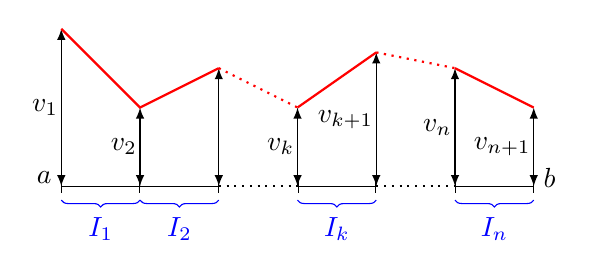
\begin{tikzpicture}
    \draw[int,|-|] (0,0) node[pt,left]{$a$}-- +(1,0) node[intname]{$I_1$};
    \draw[latex-latex] (0,0) -- node[val]{$v_1$} +(0,2) coordinate(v1);

    \draw[int,-|] (1,0) -- +(1,0) node[intname]{$I_2$};
    \draw[latex-latex] (1,0) -- node[val]{$v_2$} +(0,1) coordinate(v2);

    \draw[dotted,thick] (2,0) -- +(1,0);
    \draw[latex-latex] (2,0) -- +(0,1.5) coordinate(v3);

    \draw[int,|-|] (3,0) -- +(1,0) node[intname](Ik){$I_k$};
    \draw[latex-latex] (3,0) -- node[val]{$v_k$} +(0,1) coordinate(vk);
    \draw[latex-latex] (4,0) -- node[val]{$v_{k+1}$} +(0,1.7) coordinate(vk1);


    \draw[dotted,thick] (4,0) -- +(1,0);

    \draw[int,|-|] (5,0) -- +(1,0) node[intname]{$I_n$} node[pt,right]{$b$};
    \draw[latex-latex] (5,0) -- node[val]{$v_{n}$} +(0,1.5) coordinate(vn);

    \draw[latex-latex] (5,0) ++(1,0) -- node[val]{$v_{n+1}$} +(0,1) coordinate(vn1);

    \draw[thick, red] plot coordinates {(v1) (v2) (v3)};
    \draw[thick, red, dotted] plot coordinates {(v3) (vk)};
    \draw[thick, red] plot coordinates {(vk) (vk1)};
    \draw[thick, red, dotted] plot coordinates {(vk1) (vn)};
    \draw[thick, red] plot coordinates {(vn) (vn1)};
  \end{tikzpicture}
\end{document}
